%%PREAMBLE %%%%%%%%%%%%%%%%%%%%%%%%%%%%
\documentclass[10pt, a4paper]{article}% size of txt = 10pt
\usepackage[top= 2cm,
			bottom = 2cm,
			left = 1.7cm,
			right = 1.7cm,
			footskip = 0.5cm,
			headsep = 0cm,
			headheight = 0cm
					]{geometry}
\usepackage{amsmath} % math packages
\usepackage{amsfonts}% math packages
\usepackage{amssymb} % math packages
\usepackage{graphicx} %package for including graphics
\usepackage{array}
\usepackage[thinlines]{easytable}
\usepackage{float}
\usepackage[section]{placeins}
\usepackage[hidelinks]{hyperref}
\usepackage[shortlabels]{enumitem}
\usepackage{svg}
\usepackage{bigstrut}
\usepackage{wrapfig,lipsum,booktabs}
\usepackage{subcaption}
\usepackage{xfrac}
\usepackage{pdfpages}
\usepackage{listings}
\usepackage{xcolor}

\usepackage{listings}
\usepackage{color} %red, green, blue, yellow, cyan, magenta, black, white
\definecolor{mygreen}{RGB}{28,172,0} % color values Red, Green, Blue
\definecolor{mylilas}{RGB}{170,55,241}

\definecolor{codegreen}{rgb}{0,0.6,0}
\definecolor{codegray}{rgb}{0.5,0.5,0.5}
\definecolor{codepurple}{rgb}{0.58,0,0.82}
\definecolor{backcolour}{rgb}{1,1,1}

\lstdefinestyle{mystyle}{
    backgroundcolor=\color{backcolour},   
    commentstyle=\color{codegreen},
    keywordstyle=\color{magenta},
    numberstyle=\tiny\color{codegray},
    stringstyle=\color{codepurple},
    basicstyle=\ttfamily\footnotesize,
    breakatwhitespace=false,         
    breaklines=true,                 
    captionpos=b,                    
    keepspaces=true,                 
    numbers=left,                    
    numbersep=5pt,                  
    showspaces=false,                
    showstringspaces=false,
    showtabs=false,                  
    tabsize=2
}
\lstset{style=mystyle}


%date format
\def\mydate{\leavevmode\hbox{\twodigits\day.\twodigits\month.\the\year}}
\def\twodigits#1{\ifnum#1<10 0\fi\the#1}


\usepackage[T1]{fontenc} 
\usepackage{lmodern}
\usepackage{indentfirst}
\setlength{\parindent}{1cm}

\makeatletter
\newcommand{\thickhline}{%
    \noalign {\ifnum 0=`}\fi \hrule height 2pt
    \futurelet \reserved@a \@xhline
}
\newcolumntype{"}{@{\hskip\tabcolsep\vrule width 2pt\hskip\tabcolsep}}
\makeatother
\newcolumntype{?}{!{\vrule width 2pt}}
%%DOC ENVIROMENT%%%%%%%%%%%%%%%%%%%%%%%
\begin{document}
%Title 
\begin{flushleft}%% left justification
	\textbf{\Large{MKC-DVV: Laboratorní úloha č.6}}\hfill Filip Paul\\
	\large{Měření parametrů signálu při příjmu DAB/DAB+ \hfill\mydate}
\end{flushleft}
\section{\Large Výsledky měření:}
\begin{table}[ht!]
    \begin{minipage}{0.48\textwidth}
    \resizebox{!}{!}{%
    \begin{tabular}{|cccc|}
    \hline
    \multicolumn{4}{|c|}{\textbf{závislost SNR na C/N pro P = 20, 50 a 70 dBm}}                                                             \\ \hline
    \multicolumn{1}{|c|}{\textbf{C/N : P}} & \multicolumn{1}{c|}{\textbf{70 dBm}} & \multicolumn{1}{c|}{\textbf{50 dBm}} & \textbf{20 dBm} \\ \hline
    \multicolumn{1}{|c|}{\textbf{40}}      & \multicolumn{1}{c|}{25,4}            & \multicolumn{1}{c|}{33,5}            & 31,9            \\ \hline
    \multicolumn{1}{|c|}{\textbf{35}}      & \multicolumn{1}{c|}{25,8}            & \multicolumn{1}{c|}{31,4}            & 31,8            \\ \hline
    \multicolumn{1}{|c|}{\textbf{30}}      & \multicolumn{1}{c|}{25,2}            & \multicolumn{1}{c|}{30,7}            & 29,6            \\ \hline
    \multicolumn{1}{|c|}{\textbf{25}}      & \multicolumn{1}{c|}{24,4}            & \multicolumn{1}{c|}{27,5}            & 26,4            \\ \hline
    \multicolumn{1}{|c|}{\textbf{20}}      & \multicolumn{1}{c|}{22,6}            & \multicolumn{1}{c|}{24,4}            & 24,1            \\ \hline
    \multicolumn{1}{|c|}{\textbf{17}}      & \multicolumn{1}{c|}{20,5}            & \multicolumn{1}{c|}{21,4}            & 21,3            \\ \hline
    \multicolumn{1}{|c|}{\textbf{15}}      & \multicolumn{1}{c|}{19,2}            & \multicolumn{1}{c|}{20,1}            & 19,7            \\ \hline
    \multicolumn{1}{|c|}{\textbf{12}}      & \multicolumn{1}{c|}{16,6}            & \multicolumn{1}{c|}{17,1}            & 17,2            \\ \hline
    \multicolumn{1}{|c|}{\textbf{10}}      & \multicolumn{1}{c|}{14,7}            & \multicolumn{1}{c|}{15,1}            & 15,2            \\ \hline
    \multicolumn{1}{|c|}{\textbf{5}}       & \multicolumn{1}{c|}{10,2}            & \multicolumn{1}{c|}{10,4}            & 10,4            \\ \hline
    \multicolumn{1}{|c|}{\textbf{3}}       & \multicolumn{1}{c|}{8,5}             & \multicolumn{1}{c|}{8,5}             & 8,5             \\ \hline
    \multicolumn{1}{|c|}{\textbf{0}}       & \multicolumn{1}{c|}{6}               & \multicolumn{1}{c|}{6,1}             & 6               \\ \hline
    \end{tabular}%
    }
\end{minipage}
\hfill
\begin{minipage}{0.48\textwidth}
    \centering
    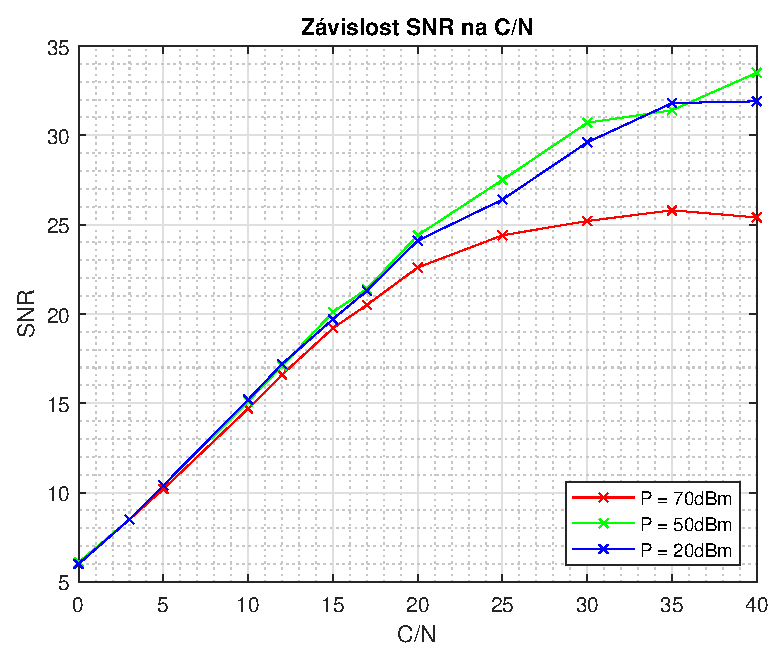
\includegraphics[width=1\textwidth]{SNR_CN.eps}
\end{minipage}

\end{table}


    % Please add the following required packages to your document preamble:
% \usepackage{graphicx}
\begin{table}[]
    \resizebox{!}{0.15\textheight}{%
    \begin{tabular}{|c|c|c|c|c|}
    \hline
    \textbf{v}  & \textbf{MOD 1} & \textbf{MOD 2} & \textbf{MOD 3} & \textbf{MOD 4} \\ \hline
    \textbf{40} & 31,6           & 32,2           & 32,4           & 32,2           \\ \hline
    \textbf{35} & 30,9           & 31,2           & 32,5           & 29,7           \\ \hline
    \textbf{30} & 30,7           & 30,5           & 30,6           & 28,6           \\ \hline
    \textbf{25} & 27,7           & 27,5           & 28,2           & 26,4           \\ \hline
    \textbf{20} & 24,6           & 24,4           & 24,4           & 23,5           \\ \hline
    \textbf{17} & 21,5           & 22             & 21,8           & 21,4           \\ \hline
    \textbf{15} & 19,8           & 19,8           & 20,1           & 20             \\ \hline
    \textbf{12} & 17,1           & 16,9           & 17,4           & 16,8           \\ \hline
    \textbf{10} & 15,1           & 15,2           & 15             & 15,2           \\ \hline
    \textbf{5}  & 10,5           & 10,4           & 10,9           & 10,2           \\ \hline
    \textbf{3}  & 8,6            & 8,5            & 8,2            & 8,8            \\ \hline
    \textbf{0}  & 6,1            & 6,1            & 6,1            & 5,8            \\ \hline
    \end{tabular}%
    }
    \end{table}

    % Please add the following required packages to your document preamble:
% \usepackage{graphicx}
\begin{table}[]
    \resizebox{!}{0.15\textheight}{%
    \begin{tabular}{|c|c|c|c|c|}
    \hline
                & \textbf{RA 4 DAB} & \textbf{RA 6 DAB} & \textbf{TU 6} & \textbf{TU 12} \\ \hline
    \textbf{40} & 21,8              & 32,7              & 29,1          & 27,7           \\ \hline
    \textbf{35} & 19,7              & 29,1              & 25,5          & 26,4           \\ \hline
    \textbf{30} & 15,5              & 28,1              & 26,4          & 26,2           \\ \hline
    \textbf{25} & 13,5              &                   & 24,7          & 24,6           \\ \hline
    \textbf{20} & 12,6              & 14,3              & 21,7          & 21,5           \\ \hline
    \textbf{17} & 10,2              &                   & 19,2          & 19             \\ \hline
    \textbf{15} & 11                &                   & 17,3          & 17             \\ \hline
    \textbf{10} & 8,4               & 10,6              & 13,7          & 14,9           \\ \hline
    \textbf{5}  & 5,5               &                   & 9,8           & 11,3           \\ \hline
    \textbf{0}  & 2,7               & 3,5               & 4,8           & 5,4            \\ \hline
    \end{tabular}%
    }
    \end{table}
\end{document}

%\[f(x)= (x+2)^2 - \frac{9\cdot 2\pi}{26}\] %%mathematic equatation in display style mode
%%optional:
%	\begin{align} %%this alignes all charakters after & if *is removed equations will be numbered
%	\hspace{5cm}  
%		 x &= a_2 x^2 +_1 x + a_0 \\
% 		x &=x^2 \nonumber		%no number will not add number to eq
%	\end{align}
